%%%%%%%%%%%%%%%%%%%%%%%%%%%%%%%%%%%%%%%%%%%%%%%%%%%%%%%%%%%%%%%%%%%%%%%%%%%%%%%%
% simulation.tex: Chapter on MC production:
%%%%%%%%%%%%%%%%%%%%%%%%%%%%%%%%%%%%%%%%%%%%%%%%%%%%%%%%%%%%%%%%%%%%%%%%%%%%%%%%
\chapter{Monte Carlo Generation}
\label{Chapt:simulation_chapter}
%%%%%%%%%%%%%%%%%%%%%%%%%%%%%%%%%%%%%%%%%%%%%%%%%%%%%%%%%%%%%%%%%%%%%%%%%%%%%%%%


\begin{chapquote}{Terry Pratchett, \textit{The Long Earth}}
"Maybe the only significant difference between a really smart simulation and a human being was the noise they made when you punched them.''
\end{chapquote}


Many theoretical models of the fundamental forces have been produced by physicists. Such models can predict the total rate or cross-section for interactions as well as, ideally, differential cross-sections as a  function of an interesting variable (such as \phistar), allowing them to be tested by comparing them to measured results.  However, some of these properties can not be calculated and some properties can not be measured directly due to limitations in experiments. These limitations include insufficient precision in measurement as well as cases where a fraction of events can not be observed by the experiment, such as when an electron is curved by the magnetic field and never reaches the detector, or cases where it travels parallel to the beam line. In these cases, applying the full theoretical calculations would require phase-space constraints and marginalizing over resolution variables in a highly complex manner.  Rather than calculating continuous distributions, the Monte Carlo method is used to generate simulated events using physics and random numbers. These numbers are drawn from distributions that are either based on theory or measured results, and are used to create a simulated event.  Simulated events can be subjected to detector simulation to model imperfections and can be processed identically to detector events. This chapter concerns the specifics of how these simulated events are created.
\section{A simple simulation example}


Here is a simple example of a simulation and the distributions used for $\ee\to\Ztomumu$. The differential cross section, assuming no higher order effects, is  
\begin{equation}\label{eq:ZDifCrossSection}
    \frac{\dir{\sigma_0(s)}}{\dir{\Omega_{\mu^-}}}
    =
    \frac{g_\Z^4s}{1024\pi^2}
    \frac{[(c_\Particle{V}^\electron)^2+(c_\Particle{A}^\electron)^2][(c_\Particle{V}^\muon)^2+(c_\Particle{A}^\muon)^2](1+\cos^2{\theta})+8c_\Particle{V}^\electron 
    c_\Particle{A}^\electron
    c_\Particle{V}^\muon
    c_\Particle{A}^\muon
    }{(s-m^2_{\Z})^2+m^2_{\Z}\Gamma^2_\Z},
\end{equation}
where $c_\Particle{V}$ and $c_{A}$ are the vector and axial coupling factors respectively, with $c_\Particle{A}^\electron=c_\Particle{A}^\muon=-0.5$ and $c_\Particle{V}^\electron=c_\Particle{V}^\muon=c_\mathrm{V}\approx-0.04$, such that
\begin{equation}\label{eq:ZDifCrossSection2}
    \frac{\dir{\sigma_0(s)}}{\dir{\Omega_{\mu^-}}}
    =
    \frac{g_\Z^4s}{1024\pi^2}
    \left[\frac{\left(c_\Particle{V}^2+\frac{1}{4}\right)^2(1+\cos^2{\theta})+2c_\Particle{V}^2}{(s-m^2_{\Z})^2+m^2_{\Z}\Gamma^2_\Z}
    \right].
\end{equation}
The variable $\Omega_{\mu^-}$ is the angular phase space of the muon.  In this case, the center of mass energy for each event ($\sqrt{s}$) could be held at the accelerator-defined value, leaving only two random variables: the azimuthal angle $\phi$ and the polar angle $\theta$ of one of the resulting muons, as they have equal and opposite momenta. The $\phi$ could be chosen from a flat distribution and $\theta$ would be taken from the differential cross section distribution. As can be seen in Fig \ref{fig:compBetweenFormulaAndRandom}, even after 100 events, the distribution of $\theta$ produced through the Monte Carlo method approaches the nominal distribution quickly.

\begin{figure}
    \centering
    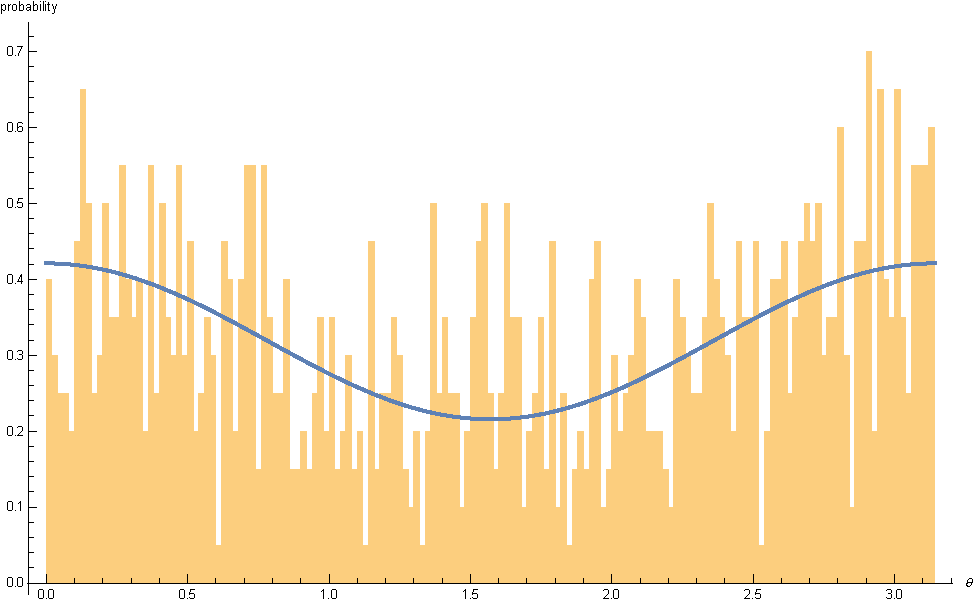
\includegraphics{figures/Simulation/compBetweenFormulaAndRandom.pdf}
    \caption[]{The probability distribution expected for the $\theta$ measurement of a \muon produced by a \Z based on Eq. \ref{eq:ZDifCrossSection2} compared to a distribution created using 100 randomly produced events using Eq. \ref{eq:ZDifCrossSection2}.}
    \label{fig:compBetweenFormulaAndRandom}
\end{figure}

In order to improve the accuracy of the simulation, Initial State Radiation (ISR) can be included, in which one the initial particles emits a photon ($\ee\to\Z\gamma\to\mumu\gamma$). This leads to a more complicated cross section as can be seen in Ref. \cite{HardPhotonCalc} where it occupies three pages of text. This example is the simplest example with one photon, and ignores situations such as when the photon is absorbed by the other electron. As additional photons are added, the complexity would increases geometrically making it  impractical to directly calculate even relatively simple interactions. 

%\section{Simulations of Hadron Collisions}
\section{Structure of a Hadron Collision Simulation}

Due to the composite nature of the projectiles in a hadron collider, simulations typically have two major pieces. The first step simulates the specific interaction using first principles with a ``generator." For the leading order (LO) case, this would mean simulating just the quarks directly creating a Z as can be seen in  Fig \ref{fig:ZSimple}. However, this is a non-physical event in that it has two quarks colliding directly rather than two protons, which contain multiple quarks as well as gluons. To complete the event, ``hadronizers" are used. These pieces of software work backwards from the quarks to describe the proton they came from and the fate of the other partons of each proton, by describing QCD interactions. The hadronizer is also responsible for describing the process by which any final state quark or gluon eventually produces a collection of observable hadrons. Such collections, whether produced in the final state of the hard scatter or the initial proton fragmentation, are called \textbf{jets}. 

\begin{figure}[!htbp]
    \centering
    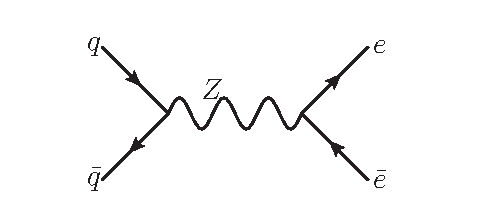
\includegraphics[width=\textwidth]{figures/DYSimple.eps}
    \caption[
        Simple \qqbar \to \Ztoee  diagram
    ]{  Simple \qqbar \to \Ztoee    }
    \label{fig:ZSimple}
\end{figure}
 Jets can be created when a large amount of energy is added to partons making up a hadron. As mentioned in Sec. \ref{sec:StrongForce}, partons must exist in a colorless state. Normally the quarks and gluons that make up a hadron such as a proton are unable to separate. However, when enough energy is added to the partons, it is possible for new quark antiquark pairs to be created, allowing quarks to leave the confines of the hadron. An example is shown in Fig. \ref{fig:Simple1Jet}, in which a photon is absorbed by a proton, which then produces a $\ensuremath{u}\Bar{\ensuremath{u}}$ pair. If enough energy is added to the system, the new particle can also create additional new particles, and so on, until all the new particles are near their ground state, leading to a collection of hadrons traveling in roughly the same direction.
 
 \begin{figure}
     \centering
     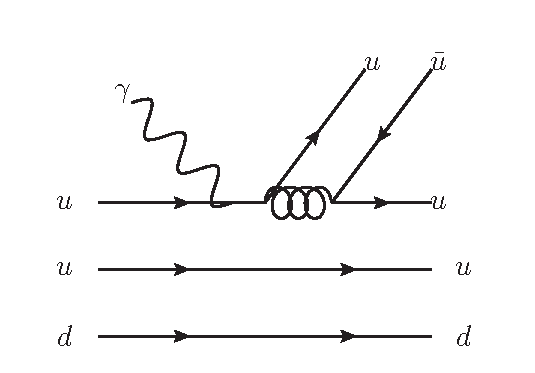
\includegraphics{figures/Simulation/Simple1Jet.eps}
     \caption{A simple example showing how energy added to a parton can produce an additional hadron}
     \label{fig:Simple1Jet}
 \end{figure}

When the hadronizer adds new particles to the simulation they are not added completely independent of the particles created by the generator. The new quarks and gluons can interact with the particles created by the generator, such as exchanging gluons or even by having the ``generator" quarks produce gluons such as in the example shown in Fig \ref{fig:HadronizationExample}. The initial quarks, labeled 0, are produced by a different generator such as \POWHEG.  The hadronizer then produces the particles in the order labeled. The choice of what particle to add and its momenta is influenced by the particular PDF that the hadronizer uses, with the PDF being called for each new particle added. These new interaction vertices are created in decreasing order of hardness, with the quark labeled 2 having the largest energy, followed by gluon 4 and so on. This is intuitive as virtual particles are only capable of existing for a very short time. When these quarks emit a gluon, they become more and more virtual, and therefore can only emit large energy particles right before they have their final interaction. These emitted gluons are capable of splitting into a $\qqbar$ pair and becoming a jet. The scale of these emissions are of the order of a few GeV. 

\begin{figure}
    \centering
    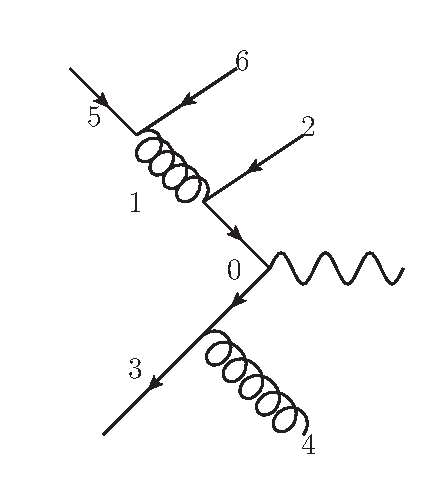
\includegraphics[width=\textwidth]{figures/Simulation/HadronizerExample.eps}
    \caption{An example showing the order of creation of particles by \PYTHIA. The 0 indexed quarks are the inputs to the system and are created by the generator, such as \POWHEG.}
    \label{fig:HadronizationExample}
\end{figure}


\subsection{PDFs and Simulations}
As mentioned before, PDFs can not be calculated from first principles. Therefore, simulation software is fed premade PDFs. Although not uncorrelated, the generator and the hadronizer do not use the same PDFs. This is partially due to the fact the PDFs are related to the energy of the interaction, and the generator and the hadronizer are inherently focused on different energy scales. Despite this, each PDF can not be chosen completely independently from the other, due to overlaps in the phase spaces of their interactions. The choice of PDF can affect the final distribution as much as changing other aspects of the simulation.

An example of the effect these parameters have is shown in Fig \ref{fig:PDFToTunesCompare}, which compares the default \Z rapidity distribution changing either the PDF of the hadronizer or the generator. As can be seen in the plot, the changes to the hadronizer do not change the rapidity distribution of the Z in a statistically significant way. However, changing the PDF of the generator creates a very noticeable change in the rapidity distribution. This is intuitive due to the difference in energy scales between the generator and the hadronizer. From Eq. \ref{eq:RapidityPDF}, changing the PDF of the generator must change the rapidity distribution. In contrast, the hadronizer, which changes the quarks momentum and therefore the Z's momentum by only a few GeV, has a minor effect on the rapidity distribution. For energies on the order of the \Z mass, the rapidity of any \Z only changes on the order of 1\% due to hadronizer effects. However the effect on the Z \pt can be larger as we will observe later. 



\begin{figure}
    \centering
    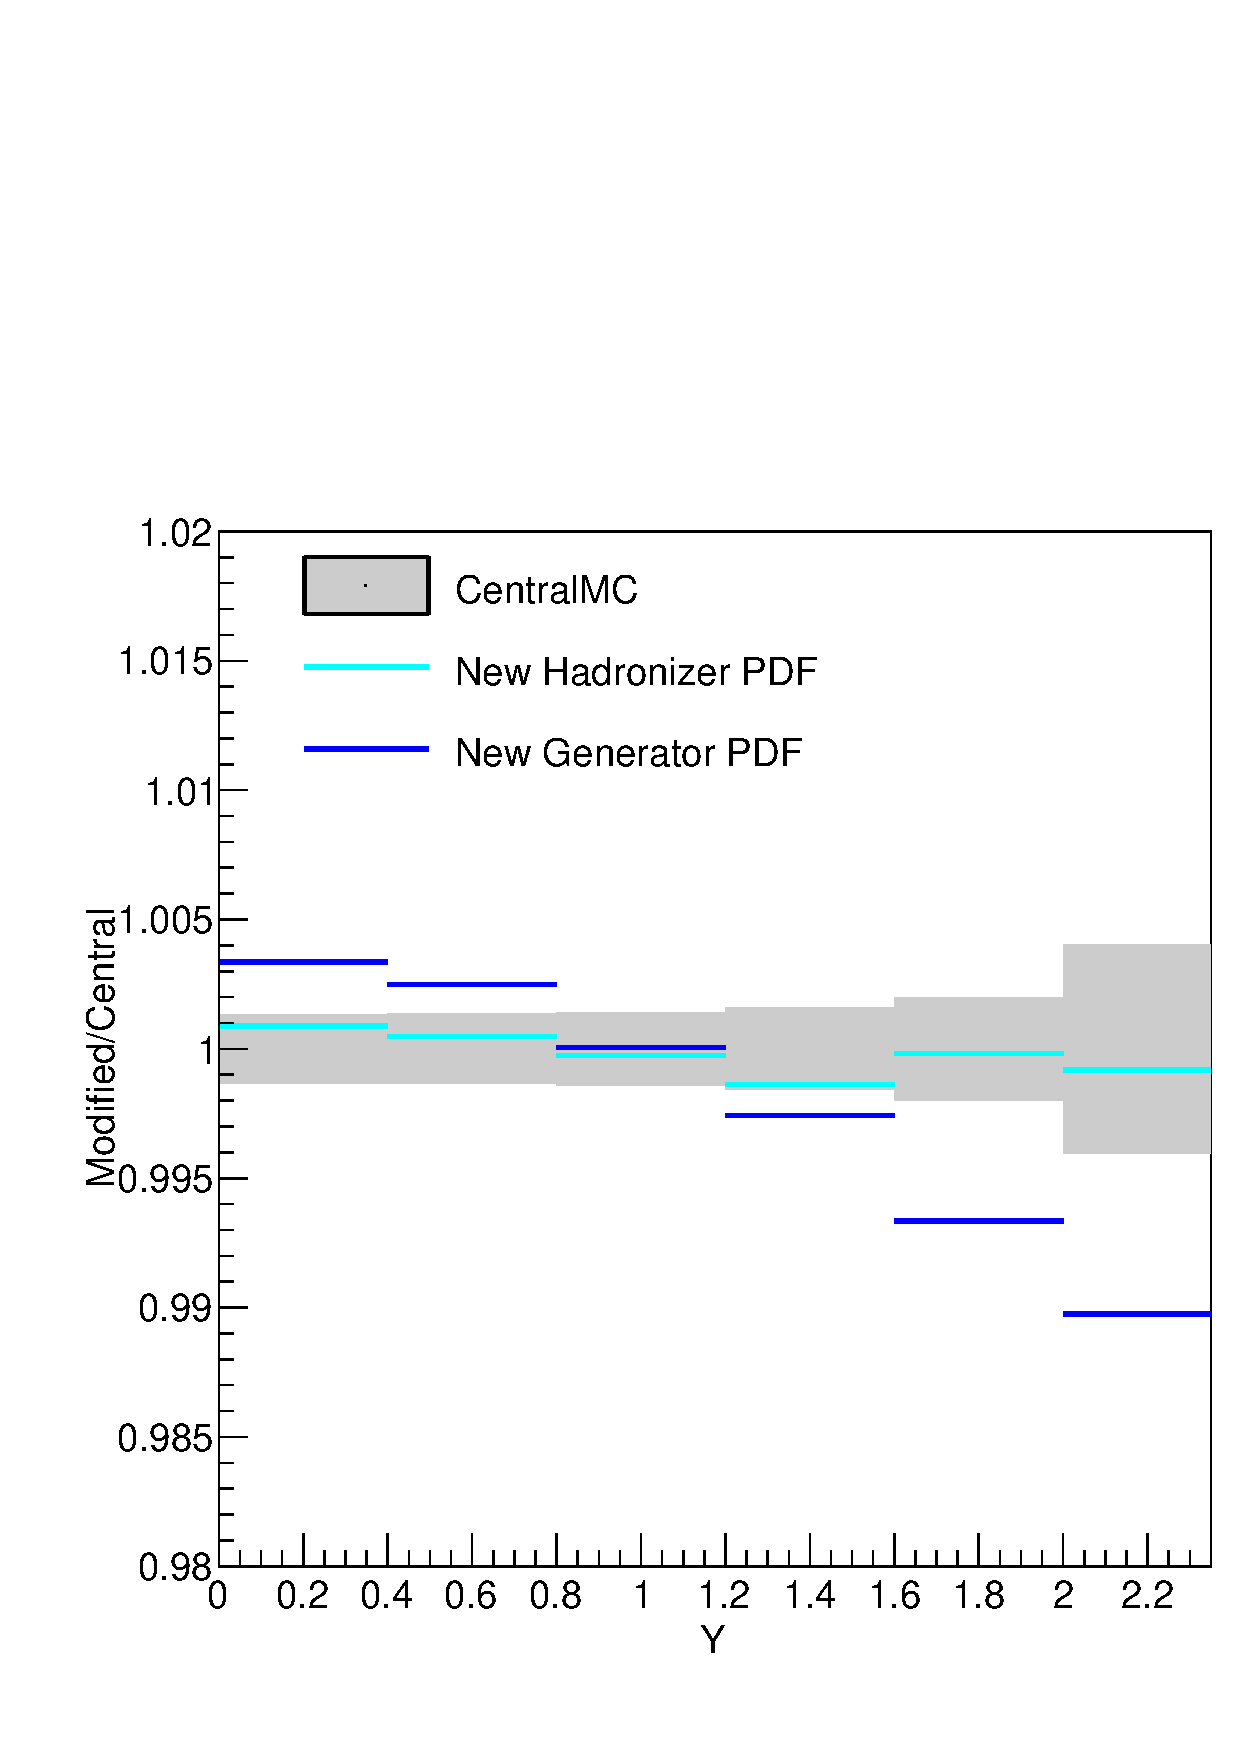
\includegraphics[width=\textwidth]{figures/Simulation/RAtioComparisons.pdf}
    \caption{This plot shows the rapididty distribution of a Z boson produced by using \POWHEG+\PYTHIAeight after changing either the PDF of \POWHEG or the PDF used by \PYTHIAeight}
    \label{fig:PDFToTunesCompare}
\end{figure}




\subsection{Higher Order simulations}\label{sec:HighOrder}

In order to increase the accuracy of the simulations, higher order generators are used. These include effects from extra gluons such as loops as shown in Fig \ref{fig:HigherOrderZSim}.
\begin{figure}[!htbp]
    \centering
   \begin{subfigure}[b]{\SideBySidePlotWidth} 
        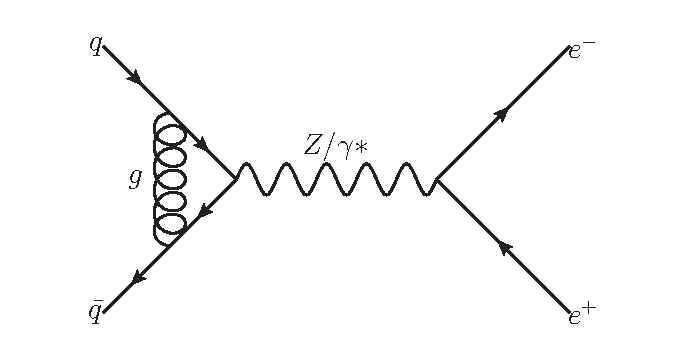
\includegraphics[width=\linewidth]{figures/DYloops.eps}
        \caption{}
        \label{fig:ZLoop1}
    \end{subfigure}%
    \begin{subfigure}[b]{\SideBySidePlotWidth}
        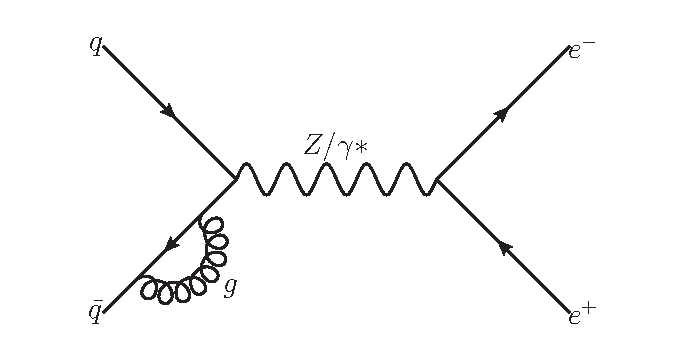
\includegraphics[width=\linewidth]{figures/DYmoreloops.eps}
        \caption{}
        \label{fig:ZLoop2}
    \end{subfigure}%
    \caption[
        The particles of the Standard Model.
    ]{
      Higher order terms of the production of a Z. These include extra gluons that are involved in the production.
    }
    \label{fig:HigherOrderZSim}
\end{figure}
The increase in accuracy comes at a cost of increased complexity. In the case of next-to-leading order (NLO) simulation, one of the most important issues involves overlap of phase-space for produced gluons of both the generator and the hadronizer. As mentioned earlier, the value of \alphastrong increases at lower energies, which limits the ability for generators to include low energy gluons. However, this lower limit is not well-defined; as \alphastrong approaches unity the higher order terms have larger and larger effects on the output, but do not have an obvious cutoff. This causes issues in the case of gluon ISR with an example shown in Fig \ref{fig:DYGFQ}. For high energy, this gluon would be produced by the generator while for low energy this gluon is produced by the hadronizer. Intrinsically there exists an area where both phases spaces overlap, leading to a nonphysical excess of these types of events. 

Multiple methods exist to correct for this overlap effect. One method has the generator create events with negative weights to cancel out this overlapping phase space. This requires knowledge of which hadronizer will be used with the output, as well as increasing the statistical uncertainty. Another method to avoid these negative weights and increase the flexibility of the hadronizers used is the Positive Weight Hardest Emission Generator (\POWHEG). Using this method, a single jet is always created with the process of interest by the generator, and is defined as the highest \pt jet in the interaction. The NLO events thus produced can then be hadronized by any hadronizer that is $\pt$-ordered. Such $\pt$-ordered hadronizers create objects so that each new object has a smaller $\pt$ than the other objects in the event, leading to $p_{\mathrm{T}1}>p_{\mathrm{T}2}>p_{\mathrm{T}3}>p_{\mathrm{T}4}$... Such a hadronizer can be combined very easily with \POWHEG since \POWHEG 's jet's $\pt=\pt_1$ by definition.

\begin{figure}[!htbp]
    \centering
    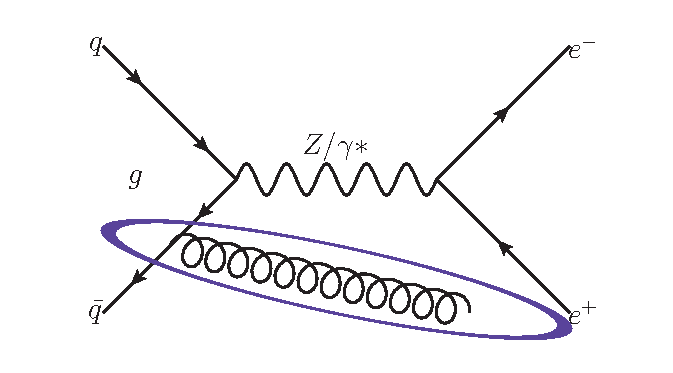
\includegraphics[width=\textwidth]{figures/Simulation/DYGluonJet.eps}
    \caption[
        The particles of the Standard Model.
    ]{
     A gluon is being emitted from one of the initial quarks. This gluon can be produced by either the generator or the hadronizer tuning.
    } 
    \label{fig:DYGFQ}
\end{figure}
\subsection{Initial State Parameters}\label{Sec:ISP}
The \PYTHIA hadronizer is the most widely used software package for this task in HEP. Hadronizers use many parameters to calculate the final state of an interaction that were created in an attempt to match data. These are referred to as ``tunes". By changing some of the values of these parameters, it is possible to attempt to better match the simulation to the data. 

 The quarks that make up a proton are in constant motion inside of it. This motion means that even when the proton is at rest, the partons that make up the proton all have some $\pt$. The $\px$ and $\py$\footnote{As was mentioned in Chapter \ref{experiment_chapter} the x coordinate points directly towards the centre of the LHC ring, and the y coordinate points directly up, and they make up the transverse plane.}  of these particles is individually chosen from a Gaussian distribution. The width of this Gaussian distribution for each parton is defined as:
\begin{equation}\label{eq:RemWidth}
\PtWidth(Q,m,y_{\mathrm{damp}};\SigmaSoft,\SigmaHard,m_{\mathrm{half}})
=
\frac{(\SigmaSoft*Q_{\mathrm{Half}}+\SigmaHard*Q)}{Q_{\mathrm{Half}}+Q}*\frac{m}{m+m_{\mathrm{half}}*y_{\mathrm{damp}}}.
\end{equation}


This contains three variables that are event dependant, $Q$, $m$, and $y_{\mathrm{damp}}$. $Q$ is the hard process renormalization, which is dependant on the individual parton interactions, $m$ the mass of the system, and $y_{\mathrm{damp}}$ is a variable that was created to damp the production of high $\pt$ at high rapidity regions. Because of limits to our detector, this study does not contain many \Z bosons of high rapidity, therefore $y_{\mathrm{damp}}$, which was created to limit effects in the high rapidity region, is small. The other four components of this equation, $\SigmaSoft$, $\SigmaHard$, $Q_{\mathrm{Half}}$, and $m_{\mathrm{half}}$, are set by the user and constant for each data set. $Q_{\mathrm{Half}}$ is the halfway point between hard and soft interactions, and $m_{\mathrm{half}}$ is the halfway point between low mass and high mass subsystem. The last two tuning parameters are $\SigmaSoft$ and $\SigmaHard$, the widths in the soft and hard interaction limits respectively. For the limiting cases, if the interaction is very hard($Q\gg Q_{\mathrm{Half}}$) then $\PtWidth\approx\SigmaHard$, while for very soft interactions($Q\ll Q_{\mathrm{Half}}$)  $\PtWidth\approx\SigmaSoft$. By changing these variables the distribution of the $\pt$ of these initial particles will change, which can effect the momentum of the \Z. In the example shown in Fig \ref{fig:HadronizationExample}, each vertex will have a different $\PtWidth$ that will be  used to calculate the momentum of the ISR particles, 6, 2, and 4.

\section{Specific production software}

%This analysis uses many different generators as well as hadronizers. The sample that was used to both unfold the data as well as estimate the efficiency was created using the generator \MADGRAPH(v1.3.30)\cite{Alwall:2011uj}.  The sample created uses the PDF set CTEQ6L1 \cite{Pumplin:2002vw}. This then uses \PYTHIAsix(v6.4.24) to hadronize the events\cite{Sjostrand:2006za}. A $k_T$-MLM Matching scheme was used \cite{Alwall:2007fs}, along with a Z* tune \cite{Chatrchyan:2013gfi, Khachatryan:2015pea} for the underlying event.
%Two centrally produced \POWHEG samples\cite{Nason:2004rx, Alioli:2010xd, Alioli:2010qp, Frixione:2007vw} were used, both using CT10NLO PDFs\cite{Gao:2013xoa}. One sample was Hadronized using \PYTHIAsix with the Z* tune, as was used with \MADGRAPH, while the other sample was hadronized with \PYTHIAeight(v8.2) \cite{Sjostrand:2014zea}. The \PYTHIAeight sample used the CUETP8M1 tune \cite{Khachatryan:2015pea} using NNPDF2.3 LO PDF \cite{Ball:2010de,Ball:2011mu}. Also used was \textsc{MadGraph5\_aMC@NLO}, commonly refered to as \AMCatNLO. This new version of \MADGRAPH is capable of creating events that are NLO accurate \cite{Alwall:2014hca}. It uses the NNPDF3.0 NLO PDF \cite{Ball:2014uwa}, and \PYTHIAeight for the parton shower and FxFx merging scheme \cite{Frederix:2012ps}. ResBos \cite{Ladinsky:1993zn,Balazs:1997xd,Landry:2002ix} with CT10NLO was used for comparisons as well.

This analysis compared unfolded data to a total of five samples. 
\begin{itemize}
    \item \MADGRAPH(v1.3.30)\cite{Alwall:2011uj}+\PYTHIAsix(v6.4.24)\cite{Sjostrand:2006za}. This sample was also used to both unfold the data as well as estimate the efficiency. The \MADGRAPH generator used the PDF set CTEQ6L1 \cite{Pumplin:2002vw}.  A $k_T$-MLM matching scheme was used \cite{Alwall:2007fs}, along with a Z* tune \cite{Chatrchyan:2013gfi, Khachatryan:2015pea} for the underlying event.
    \item \textsc{MadGraph5\_aMC@NLO}+\PYTHIAeight(v8.2).  \textsc{MadGraph5\_aMC@NLO}, commonly referred to as \AMCatNLO. This new version of \MADGRAPH is capable of creating events that are NLO accurate \cite{Alwall:2014hca}. \PYTHIAeight used the CUETP8M1 tune \cite{Khachatryan:2015pea} using NNPDF2.3 LO PDF \cite{Ball:2010de,Ball:2011mu}. 
    \item \POWHEG+\PYTHIAsix. The \POWHEG sample\cite{Nason:2004rx, Alioli:2010xd, Alioli:2010qp, Frixione:2007vw} used a CT10NLO PDF\cite{Gao:2013xoa}. It  was then  hadronized using \PYTHIAsix with the Z* tune, as was used with \MADGRAPH+\PYTHIAsix.
    \item \POWHEG+\PYTHIAeight(v8.2). The same \POWHEG sample was also used for the \POWHEG+\PYTHIAsix was hadronized with \PYTHIAeight. The settings for \PYTHIAeight were the same as for \textsc{MadGraph5\_aMC@NLO}+\PYTHIAeight(v8.2).
    \item ResBos \cite{Ladinsky:1993zn,Balazs:1997xd,Landry:2002ix} with CT10NLO
\end{itemize}

\subsection{MadGraph and aMC@nlo}

\MADGRAPH is a very commonly used  generator. It is very flexible, in that it can be given a theoretical model and produce samples based on it. It does this by calculating every possible Feynman diagram for the process of interest, to LO, or in the case of \AMCatNLO, NLO level. These are then used to create the matrix elements. This LO matrix element generator can include up to 4 extra partons in its calculation.  When creating events at NLO however, \AMCatNLO does create negative weights as was covered in Sec \ref{sec:HighOrder}.
\subsection{POWHEG}
The \POWHEG generator is a NLO calculator. However unlike \MADGRAPH, it always produces one and only one extra parton that becomes the hardest jet in the interaction. For this reason it tends to be more inaccurate in producing \Z bosons with high \pt. This is because it limits the boost that the \Z can get from partons since it is not possible to have multiple high energy jets going in the same direction that would boost the \Z in the opposite direction. This leads to a deficit of high \pt \Z events.
\subsection{RESBOS}
Unlike the other generators used, this generator does not require a hadronizer. In fact this generator does not produce single gluons but instead calculates the overall effect of all orders of gluon loops on the final product \cite{Ladinsky:1993zn,Balazs:1997xd,Landry:2002ix}. As mentioned earlier $\alphastrong > 1$ for low energy interactions, making it impossible to just consider interactions with a finite number of gluons. However, this method's weakness is that it does not have individual gluons to make jets, and in fact does not have individual particles in an event. Rather it just outputs the value of interest, in our case \phistar.   
%%%%%%%%%%%%%%%%%%%%%%%%%%%%%%%%%%%%%%%%%%%%%%%%%%%%%%%%%%%%%%%%%%%%%%%%%%%%%%%%
\section{Pileup Simulation}
\label{Sec:SimRecon}
On top of the complexities of producing the interaction of interest, the simulation must predict what the detector would have seen. This is normally done with \GEANTfour \cite{agostinelli2003} which predicts detector responses. This, however, only simulates a single pp collision. As mentioned in section \ref{Sec:Pileup}, in most events multiple protons interact, around 20 pairs for this data-set. These interactions can lead to the production of a large number of charged particles that can contaminate signal and lower its probability to be accurately reconstructed. 
\begin{figure}
    \centering
    \begin{subfigure}[b]{\SideBySidePlotWidth} 
        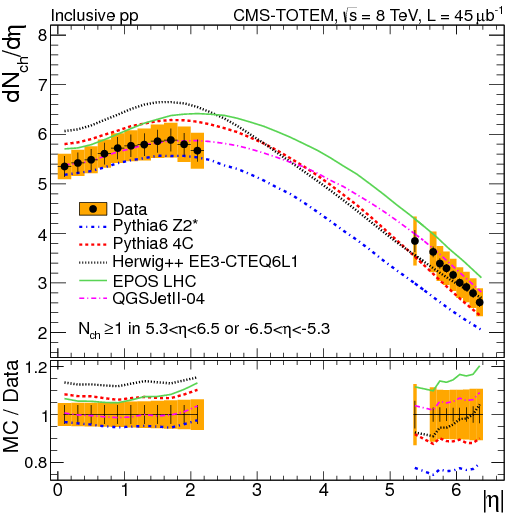
\includegraphics[width=\linewidth]{figures/Simulation/EtaPileupDist.png}
        \caption{}
    \end{subfigure}%
    \begin{subfigure}[b]{1.\SideBySidePlotWidth}
        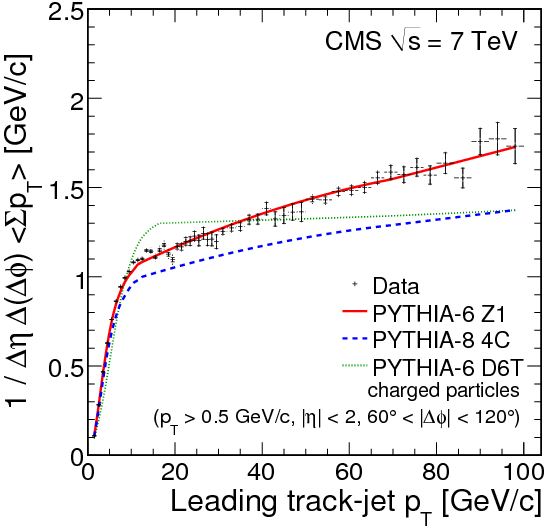
\includegraphics[width=\linewidth]{figures/Simulation/PtunderlyingEvent.png}
        \caption{}
    \end{subfigure}%
    \caption{The left figure shows the density of charged particles produced from a pp collision in a normal minbias event \cite{Chatrchyan:2014qka}. The right plot shows the average transverse energy emitted perpendicular to the largest jet of an interaction as a function of the largest jet \pt.\cite{Chatrchyan:2011id}}
    \label{fig:MinBiasFigures}
\end{figure}

In order to simulate an event accurately, simulated pileup events are added to the event. This is done using \PYTHIA to create collections of soft interactions, in which two protons hit and produce large collections of low energy particles, mostly pions. The number of these interactions that are added  to an event is taken from a distribution that was created before the data was taken. For this reason the pileup distribution does not perfectly match the measured pileup distribution. An example of this is shown in Fig \ref{fig:PileupToData}. As can be seen, both the position and shape of the distributions are different. This does not mean that on an event-by-event basis anything is wrong, rather that the rate of these events is incorrect. To more accurately reflect the pileup distribution taken from data, events are re-weighted, with the weight being the ratio of the data events over the number of Monte Carlo events in a particular bin. The data distribution was calculated using the instantaneous luminosity and the inelastic proton-proton cross-section, with the weight being the data pileup distribution over the Monte Carlo pileup distribution. 

\begin{figure}[!htbp]
    \centering
    \begin{subfigure}[b]{\SideBySidePlotWidth} 
        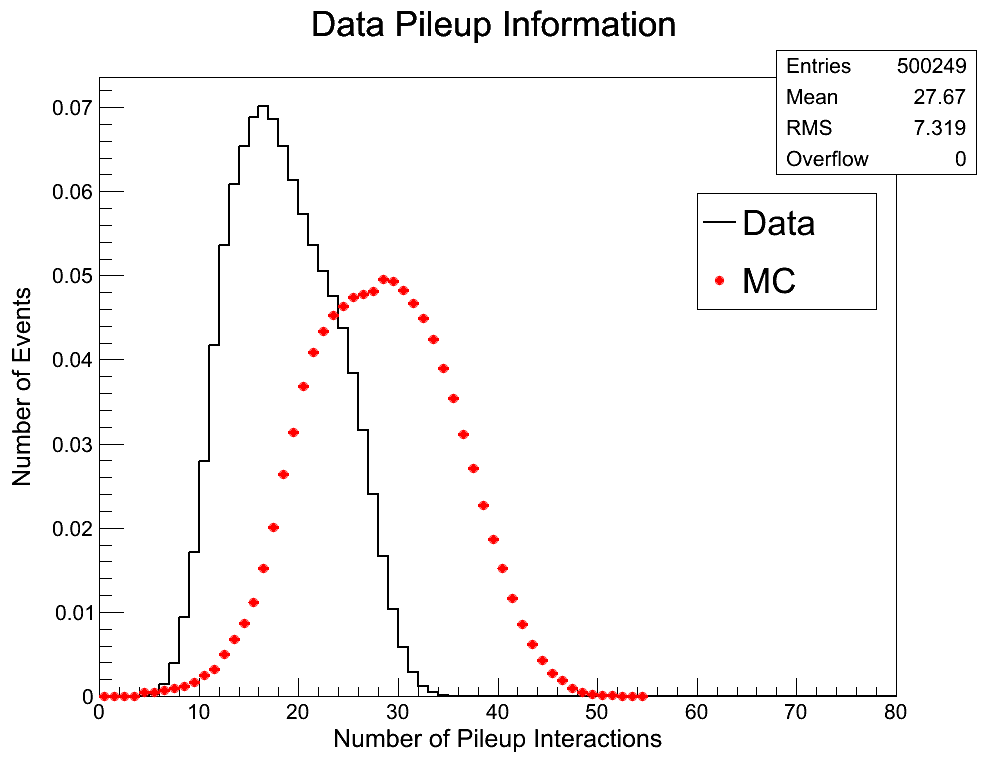
\includegraphics[width=\textwidth]{figures/Simulation/h_DataMCBCComparsionBornPt25to250.png}
        \caption{}
    \end{subfigure}%
    \begin{subfigure}[b]{\SideBySidePlotWidth} 
        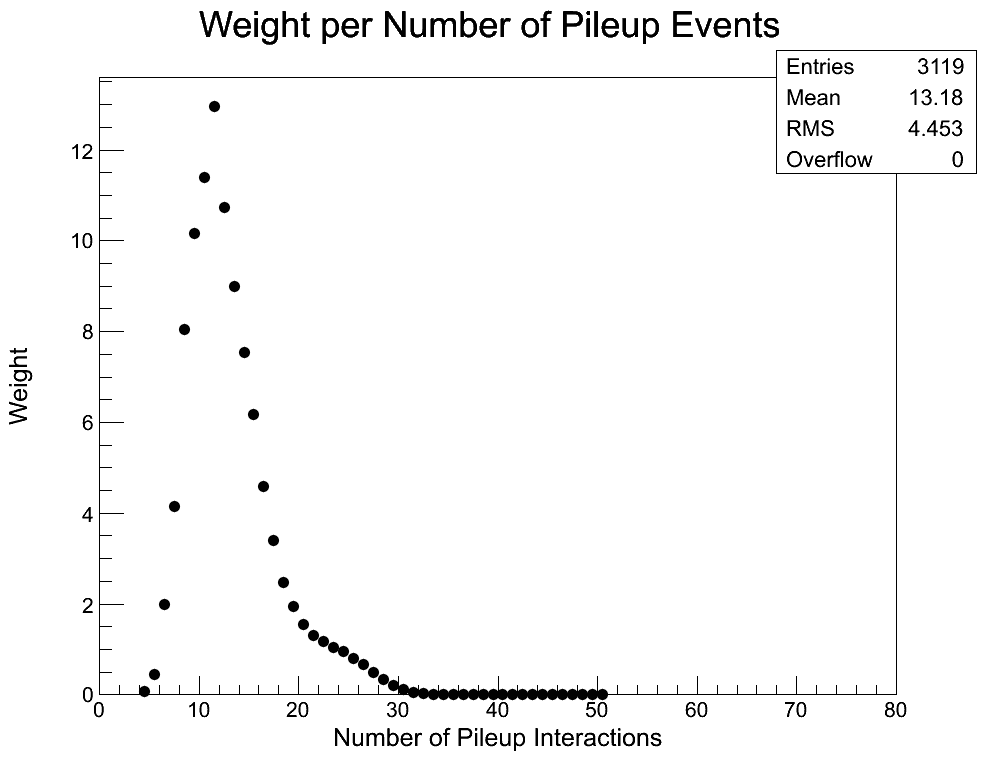
\includegraphics[width=\textwidth]{figures/Simulation/h_MCWeightsperPileUpBornPt25to250.png}
        \caption{}
    \end{subfigure}%
    \caption{The left plot compares the number of vertices per an event for Monte Carlo compared to data, while the right plot shows the resulting weights.}
    \label{fig:PileupToData}
\end{figure}

